\documentclass[11pt,a4paper]{article}

%\usepackage[a4paper,left=35mm,right=30mm,top=30mm,bottom=30mm]{geometry}
\usepackage[utf8x]{inputenc}
\usepackage[english]{babel}
\usepackage{amsmath}
\usepackage{graphicx}
\usepackage{url}
\usepackage{booktabs}
\usepackage{colortbl}
\usepackage{xcolor}
\usepackage{array} 
\usepackage{listings}
\usepackage{hyperref}
\usepackage{longtable}
\usepackage{placeins}
\usepackage[T1]{fontenc}
\usepackage{epstopdf}

\parindent 0pt

\newcommand{\changefont}[3]{
\fontfamily{#1} \fontseries{#2} \fontshape{#3} \selectfont}

\newcommand*{\todo}[1]{\textcolor{red}{[TODO: #1]}}
\newcommand*{\code}[1]{\lstinline|#1|}

\hypersetup{pdftex=true, colorlinks=true, breaklinks=true,linkcolor=black,citecolor=black}


	% Floatpage stuff
    \renewcommand{\topfraction}{0.9}	% max fraction of floats at top
    \renewcommand{\bottomfraction}{0.8}	% max fraction of floats at bottom
    %   Parameters for TEXT pages (not float pages):
    \setcounter{topnumber}{2}
    \setcounter{bottomnumber}{2}
    \setcounter{totalnumber}{4}     % 2 may work better
    \setcounter{dbltopnumber}{2}    % for 2-column pages
    \renewcommand{\dbltopfraction}{0.9}	% fit big float above 2-col. text
    \renewcommand{\textfraction}{0.2}	% allow minimal text w. figs
    %   Parameters for FLOAT pages (not text pages):
    \renewcommand{\floatpagefraction}{0.7}	% require fuller float pages
	% N.B.: floatpagefraction MUST be less than topfraction !!
    \renewcommand{\dblfloatpagefraction}{0.7}	% require fuller float pages

\begin{document}
\changefont{pbk}{m}{n}

\title{Documentation: \\ -------------------------------- \\ BuriTrack \\ --- \\ CeTrAn}
\date{\today}
\maketitle
\begin{center}
\begin{figure}[h]
	\centerline{
    	\mbox{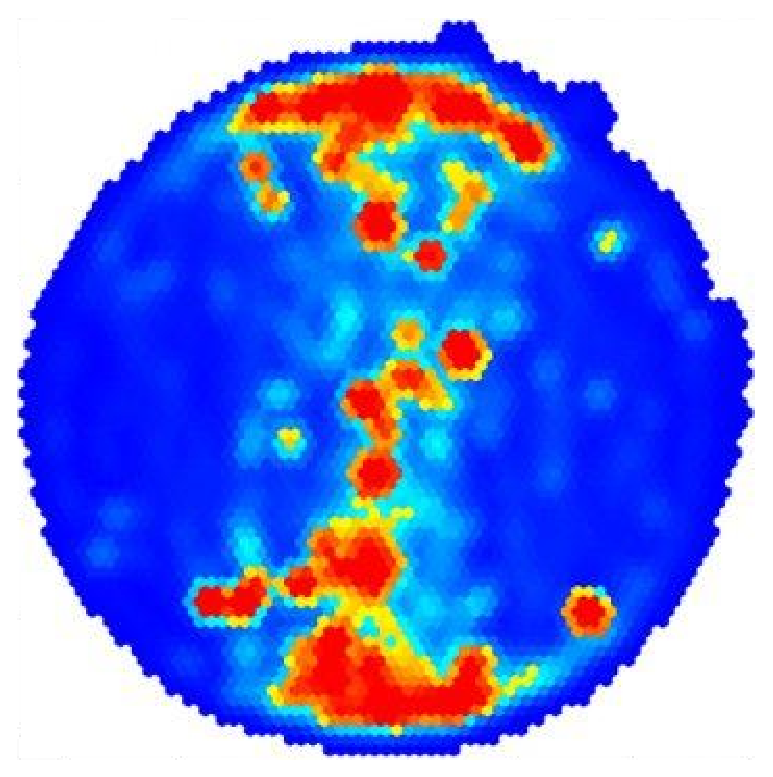
\includegraphics[width=0.5\textwidth]{figures/occupancy_plot.eps}}
  	\label{fig:title}
	}
 \end{figure}
\parskip 1cm
Project Homepage: \\
\url{http://sourceforge.net/projects/buridan/} \\
Project video:\\
\url{http://www.youtube.com/watch?feature=player_detailpage&v=YwGUlgiGcg4}
\end{center}

\thispagestyle{empty}
\newpage

\tableofcontents

\newpage

\begin{abstract}
This freeware package offers the tools to track a fly (buritrack) in the Buridan's assay and to analyse the recorded trajectories with different statistical methods (CeTrAn). The tracker may use a live picture stream from a video camera or pre-recorded videos. Since the analysis tools are written in R, they can easily be edited and customised to a user's specific needs. Furthermore, the analysis tools presently offer analyses of single flies as well as comparative analyses between groups of flies.  

Please refer to the scientific paper you will find with your download for scientific question and a better explanation of the analysis.
\end{abstract}

\section{BuriTrack}

\begin{figure}[h]
    	\mbox{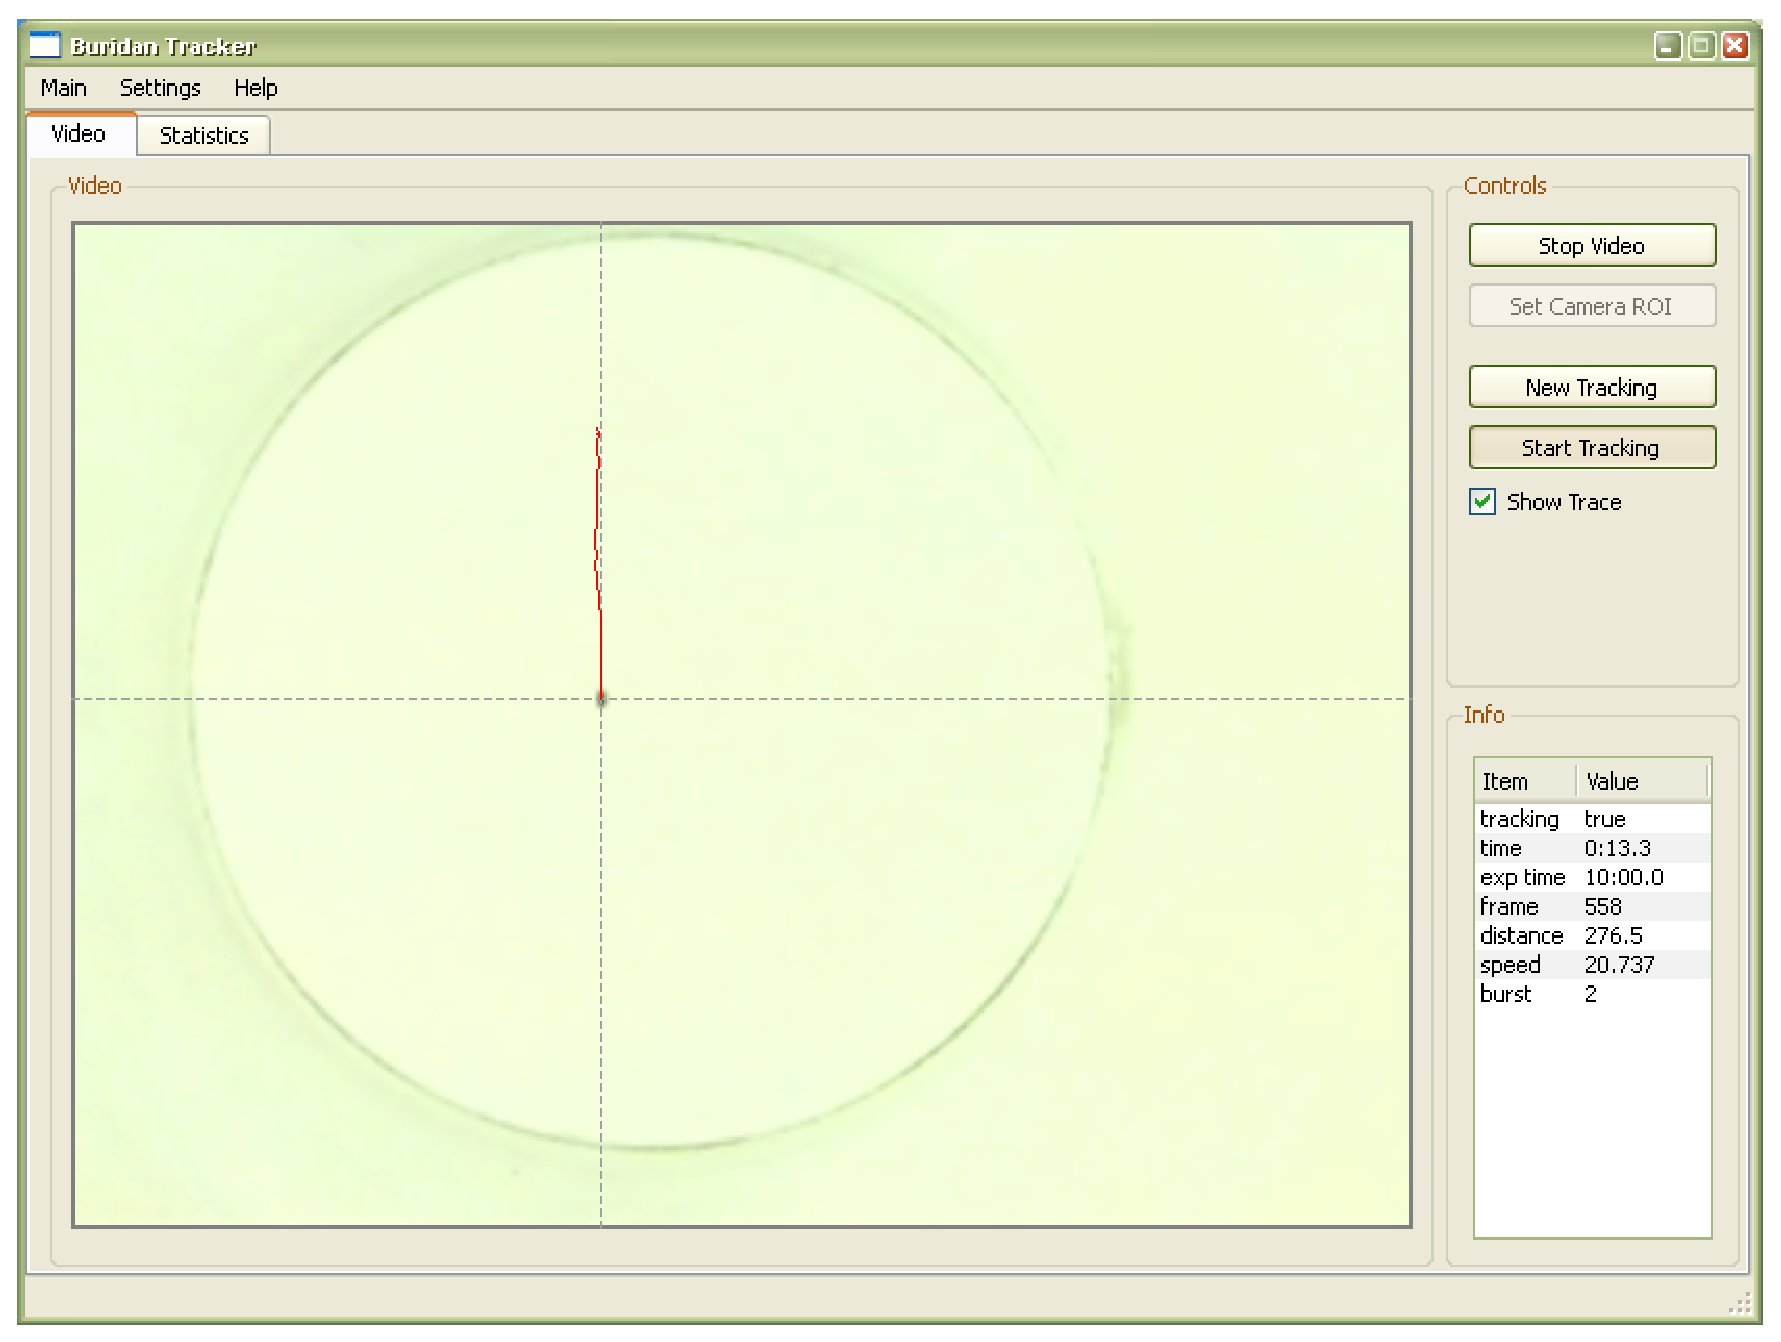
\includegraphics[width=0.99\textwidth]{figures/tracker_mainscreen.eps}}
 	\caption{The main window of BuriTrack.}
  	\label{fig:mainscreen}
 \end{figure}

\subsection{Installation}

\begin{enumerate}
\item Download the tracker from the sourceforge website. Built versions of the tracker are available for Windows and OSX. 
\item Unzip the file. 
\item Copy the folder to your preferred location on your filesystem.
\item Run the executable.
\end{enumerate}

\subsection{Compiling from source}

\subsubsection{Windows}

\begin{enumerate}
\item Install the latest versions of QT and Qt Creator: \\ \url{http://qt.nokia.com/products/developer-tools/}
\item Install the latest versions of OpenCV. We recommend MinGW (Minimalist GNU for Windows) to compile the OpenCV source \\ \url{http://opencv.willowgarage.com/wiki/} \\
Help provided by Willowgarage can be found here: \\ 
\url{http://opencv.willowgarage.com/wiki/InstallGuide} 
\item Edit the {\bf .pro} file to set your path variables. 
\end{enumerate}

\subsubsection{OSX}

This section describes the basic steps of how to compile {\it Buridan} using Qt Creator on Mac OS X. These instructions can be easily generalised to other UNIX- or Linux-based systems. 

\begin{enumerate}
\item We recommend to install the latest versions of QT and Qt Creator: \\ \url{http://qt.nokia.com/products/developer-tools/}
\item Compile the latest version of OpenCV. We recommend using MacPorts (an easy to use system for compiling, installing, and managing open source software) to install OpenCV \\ \url{http://www.macports.org/}
\item Edit the {\bf .pro} file to set your path variables. 
\end{enumerate}

\subsubsection{Linux}

Under construction.  

\subsection{Getting started}

\begin{enumerate}
\item Load a video or capture from a webcam by clicking on \\ 
Main->"New Video Capture". \\
The contrast and luminosity of your camera may need to be adjusted, such that the arena is visible.
\item Set the camera ROI (Region Of Interest) by clicking on the button.
\item Press the Button "New Tracking" and adjust all the parameters in the Tracking dialog. While setting the platform position left-click on three points on the platform edge. Check that the drawn circle fits with the platform, if not you can right-click on the mouse to erase one point (one per click).
\item Put a fly in the arena, you may want to adjust the luminosity of your camera again, such that the platform become nearly invisible. Click on "Activate Tracking". 
\end{enumerate}

To start a new tracking before the end of the experiment, deactivate the tracker by clicking "Activate Tracking" again and press the button "New Tracking". If the fly jumps off of the platform, the tracker stops and plays a sound alarming the experimenter. Put the fly back on the platform using a brush and click "Activate Tracking" again to continue with the experiment.

Once the experiment is over, you can simply start a new one by clicking the  "New Tracking" button. Note that you should either wash the platform or rotate it between experiments in order to control for  any chemical cues the flies might have left on the platform.

\subsection{Troubleshooting}

Should you get an address exception error, when starting the program, we recommend installing the Microsoft Visual C++ 2010 Redistributable Package. \\ \url{http://www.microsoft.com/download/en/details.aspx?id=8328}

Regarding any other issues you may encounter, please use the sourceforge project website \\
\url{http://sourceforge.net/projects/buridan/support} \\
or alternatively you can email {\bf jwessnit@users.sf.net}. 

\newpage
\section{CeTrAn}

\begin{figure}[h]
    	\mbox{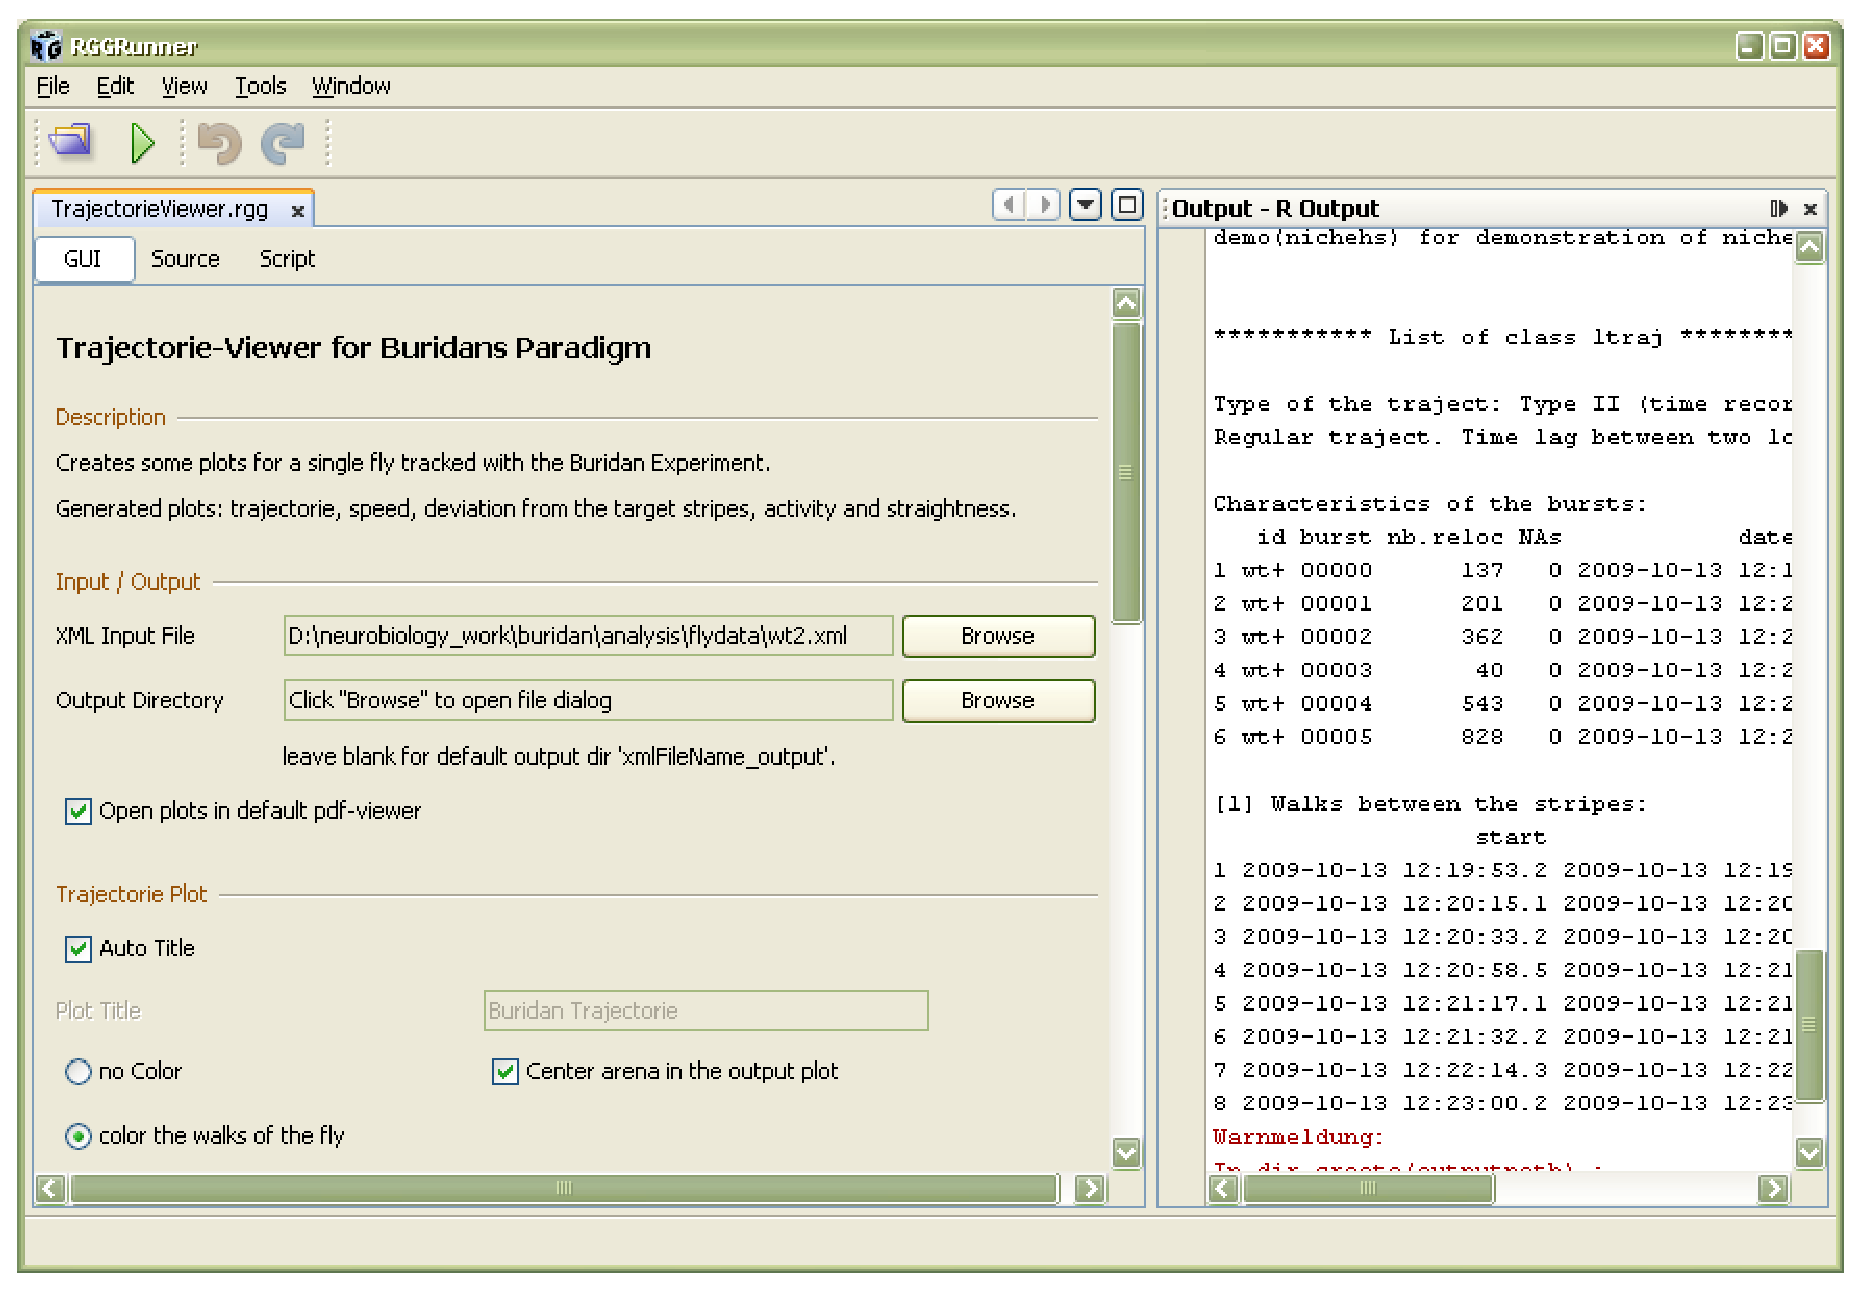
\includegraphics[width=0.99\textwidth]{figures/analysis_trajviewer.eps}}
 	\caption{The graphical user interface of CeTrAn.}
  	\label{fig:CeTrAn}
 \end{figure}

\subsection{Installation}


Tested version: install an up to date versions
\begin{enumerate}
\item Download and install the latest version of R (was tested with R3.0.0): \\
\url{http://www.r-project.org/}
\item Download and install the Rggrunner \\ \url{http://rgg.r-forge.r-project.org/downloads.html}. \\  Detailed instructions can be found here: \\
\url{http://rgg.r-forge.r-project.org/gettingstarted.html})
\item Start R GUI (Windows: start the R.exe, Linux: type "R" in console), open the file in the installation folder "install\_packages.r", and run the code.

\end{enumerate}
Should be easy and fast, but I haven't tested it yet and the installer present are for the windows version only.
\begin{enumerate}
\item Install R and the rggrunner (windows version of the installers are in the "`installation"' folder): \\

\item Copy the "`R"' folder into your document folder (windows) or your /library folder (mac) \\

\item Do NOT run the "install\_packages.r" code or update the packages.

\end{enumerate}

On Linux systems you need to install the dev packets of libxml2 first.
(more information here: \\ \url{http://cran.r-project.org/web/packages/XML/index.html})

\subsection{Getting started with data from Buritrack}

\begin{enumerate}
\item Start the Rggrunner (in windows start: <rgg\_directory>/bin/rggrunner.exe)

\item Click "`Open RGG"' and load the CeTrAn/CeTrAn\_fromxml\_4.rgg

\item Follow the instructions of the GUI. You have to choose the folder containing the data, the {\bf .txt} file linking the data with group names, and the output folder. The name of your output can be changed using the top entry field.
You can then choose which analysis you want to do, in particular you can choose if you want to have the single fly analysis or not. If you get error messages, try to do the analysis without the PCA which is the least stable code. Some limit value has to be given at the bottom: this will be used as y limit value to draw the graphs. 

\item Press the green arrow in the toolbar to execute the script.

\end{enumerate}

As stated above, you need a {\bf.txt} file with two tab separated columns. The first column contains the XML filenames of the data files, the second column contains a string which represents the group the file belongs to. You can load the file via the "Browse" button found underneath the matrix box.

\medskip 

This is an example of what your file should contain:

\begin{lstlisting}
--------------
tbh1.xml	tbh
tbh2.xml	tbh
wt+1.xml	wt+
wt+2.xml	wt+
--------------
\end{lstlisting}

NB: you can also get data that is stored in different folders by choosing the folder containing the data
as the parent folder, and adding the subfolder to the data name, as in this example:

\begin{lstlisting}
--------------
nostripe/cs_1.xml	nostripe_cs
withstripes/cs_1.xml	stripe_cs
--------------
\end{lstlisting}

\subsection{CeTrAn with other data}

This is still in development. Some scripts in the "`other\_codes"' folder may help you to modify your data such that CeTrAn can use it, you then need to use the CeTrAn\_import\_4.rgg file. The data should be in 4 columns: time in seconds, x coordinate in mm, y coordinate in mm, burst.

The way the metadata should be is still work in progress. The minimum is the path to the data, a group entry and a time stamp in this format: YYYY-MM-DD HH:MM:SS
More to come, we hope.

\subsection{Function list (not exhaustive)}

What follows is a brief outline of functions and metrics that are calculated by the CeTrAn package. 

Please refer also to the PlosOne paper. The manuscript can be found in the documentation. More detailed descriptions can be found there.

{\bf IMPORTANT:} The package contains a number of functions to analyse the trajectorie files. The first step is always to load and interpolate the trajectorie of the flies in a trajectory with a regular time difference of 100 ms (10 Hz) between all relocations. Movement smaller than the threshold value given in the GUI are eliminated.

\subsubsection{Individual test}
\label{sec:individualTest}

In the individual test pdf output, the trajectory of each fly in drawn. The color of the path changes after each walk, which eases the visualisation of the path. A histogram of the frequency of speed is also drawn on a logarithmic scale on the x axis. The next plot shows the speed over time. Next, the relative angle over time is shown where the color of the point represent the speed at that moment (also represented at the bottom with the same color code: black is slow, green is very fast.) The next histograms are self explanatory while the last one represents the absolute turning angle in red, and the absolute meander in green. 


\subsubsection{Speed}

The speed is only measured when the fly is moving, which means if $|\Delta x| + |\Delta y| > 0 $. If the speed between two relocations is higher than 50 mm/s, it is assumed the fly jumped and the speed is disregarded from the median of speed calculation.


\subsubsection{Stripe deviation}

For the stripe deviation, the absolute angle of every relocation is read. For each position of the fly, we calculate the direction of the vector pointing from the fly's position towards all the black stripes. 

If we take the angular difference between the fly's heading angle and the direction of the vectors pointing towards the stripes, we get the deviation from the middlepoints of the black stripes. Now we just find the stripe with the smallest deviation for each point and plot it in a histogram. This plot is not returned, the median value is returned for each fly. 

\subsubsection{Activity}

For now, please refer to the paper.

\subsubsection{Turning angle}

For now, please refer to the paper.

\subsubsection{Calculation of the walks between the stripes}

For each stripe, we calculate a 2D plane (straight line) orthogonal to the vector between the arena middlepoint and the stripe position. The plane lies between the arena-middlepoint and the arena border (We took a distance of 0.8*arena-radius). Whenever the fly leaves the area defined by the transecting plane and arena border, the walk is started, if it passes any other plane, the walk is completed. The walks are stored together with the time and walk distance between passing the planes.

\subsubsection{Transition plot}

The transition plot is done with the {\it hexbin} package. The Arena is divided into 60*60 hexagons. The fly's current position raises the count of its corresponding hexagon by one. The matrix is smoothed with a Gaussian kernel and then plotted. You can untipped one box if you want all data to be taken into account, the default is to use position point only if the fly was moving at that time, such that long stays do not appear in the plot.

The scale starts at 0 (blue) and goes up till a value calculated by the 95\%-quantile of the count-distribution (red). This scale makes small differences clearly visible and leaves only a few spots (5\%), which are above the scale. 

\subsection{Troubleshooting}

Regarding any other issues you may encounter, please use the sourceforge project website \\
\url{http://sourceforge.net/projects/buridan/support} \\
or alternatively you can email {\bf thrawny@users.sf.net}. 

\newpage 

\section{Buridan's assay}
On the next pages, we provide drawings by Reinhard Wolf for the Buridan's arena. We hope to provide better blueprints in the future. 

\begin{figure}[h]
    	\mbox{\includegraphics[width=0.99\textwidth]{figures/Buridan_assay-01.eps}}
 	\caption{....}
  	\label{fig:buridan-01}
 \end{figure}

\begin{figure}[h]
    	\mbox{\includegraphics[width=0.99\textwidth]{figures/Buridan_assay-02.eps}}
 	\caption{....}
  	\label{fig:buridan-02}
 \end{figure}
 
 \begin{figure}[h]
    	\mbox{\includegraphics[width=0.99\textwidth]{figures/Buridan_assay-03.eps}}
 	\caption{....}
  	\label{fig:buridan-03}
 \end{figure}
 
 \begin{figure}[h]
    	\mbox{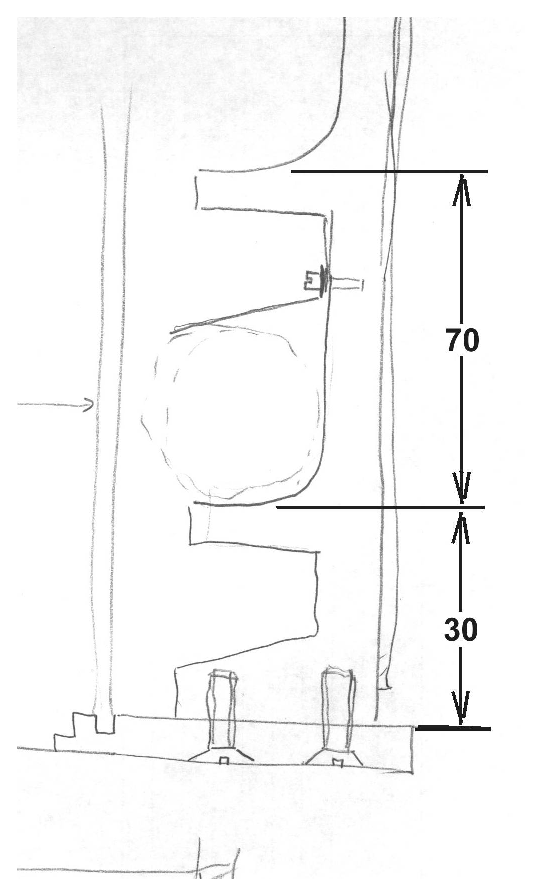
\includegraphics[width=0.9\textwidth]{figures/Buridan_assay-04.eps}}
 	\caption{....}
  	\label{fig:buridan-04}
 \end{figure}

\end{document}